% personal latex template

% vegito2002@gmail.com
\documentclass{article}
\usepackage{times}
\usepackage{mathptmx}
\usepackage{multirow}
\usepackage{enumitem}
\usepackage[letterpaper, margin=1in]{geometry}
\usepackage{hyperref}
\usepackage{amsmath}
\usepackage{mathtools}
\DeclarePairedDelimiter{\ceil}{\lceil}{\rceil}
\DeclarePairedDelimiter{\floor}{\lfloor}{\rfloor}
\usepackage{graphicx}
\usepackage{listings}
\usepackage{lipsum}
\usepackage{courier}
% \usepackage{tabularx}
\usepackage[export]{adjustbox}
% \usepackage[landscape]{pdfpages}
\usepackage{enumitem}
\usepackage{spreadtab}
% \usepackage{enumerate}


\graphicspath{ {images/} }

\usepackage[dvipsnames]{xcolor}  %% Allow color names
\lstset
{ %Formatting for code in appendix
  belowcaptionskip=1\baselineskip,
  xleftmargin=\parindent,
  language=Java,   %% Change this to whatever you write in
  breaklines=true, %% Wrap long lines
  basicstyle=\ttfamily,
  % numbers=left,
  % stepnumber=1,
  commentstyle=\itshape\color{Gray},
  stringstyle=\color{Orange},
  keywordstyle=\bfseries\color{WildStrawberry},
  identifierstyle=\color{Blue},
}
\usepackage{titlesec}
\usepackage{amssymb}
\newenvironment{claim}[1]{\par\noindent\underline{Claim:}\space#1}{}
\newenvironment{claimproof}[1]{\par\noindent\underline{Proof:}\space#1}{\leavevmode\unskip\penalty9999 \hbox{}\nobreak\hfill\quad\hbox{$\blacksquare$}}

\setcounter{secnumdepth}{4}

\titleformat{\paragraph}
{\normalfont\normalsize\bfseries}{\theparagraph}{1em}{}
\titlespacing*{\paragraph}
{0pt}{3.25ex plus 1ex minus .2ex}{1.5ex plus .2ex}

\begin{document}

% Article top matter
\title{\textsc{Project Writeup}\\ \textbf{\textsc{Multi-Diff}}}
\author{Guoye Zhang, Qiang Zhang}
\date{\today}
\maketitle

\section{Introduction}
The utility \texttt{diff} is commonly used in all scenarios, whether for programming purposes or in general text editing circumstances. Version control systems such as git integrated \texttt{diff} as a part of their core functionality. This legacy utility is based on the renowned \textit{Edit Distance} algorithm, which in essence is a Dynamic Programming algorithm. \\

Aside from the application domain of version control, \texttt{diff}'s algorithm in itself is interesting and instructive enough for most computer science students to delve into. In general sense, the concepts of finding similar text and displaying minimum edit distance can be embodied in various domains and categories of applications. Our project aims at extending \texttt{diff} to provide firstly the feature of multi-file comparison, accompanied with visualization, that can display the chain of editing among more than two related files, together with a better algorithm that fixes certain scenarios where the normal \texttt{diff}'s Edit Distance algorithm would perform suboptimally, which are cases we already described in our proposal.\\

\subsection{Algorithmic Optimization}
As a reminder, recall the scenario where normal \texttt{diff} would perform suboptimally. In this code snippet:\\
\begin{lstlisting}
   for(int i=0; i<10; i++) {
       System.out.println("First line");
   }
   for(int i=0; i<10; i++) {
       System.out.println("Second line");
   }
   for(int i=0; i<10; i++) {
       System.out.println("Third line");
   }
\end{lstlisting}
from which we will delete the second \texttt{for} block. And if we use the traditional \texttt{diff} on the old and new versions of this snippet, we would get:\\
\pagebreak
\begin{lstlisting}
   for(int i=0; i<10; i++) {
       System.out.println("First line");
   }
   for(int i=0; i<10; i++) {
 -     System.out.println("Second line");
 - }
 - for(int i=0; i<10; i++) {
       System.out.println("Third line");
   }
\end{lstlisting}
Instead of what would be expecting as follows:
\begin{lstlisting}
   for(int i=0; i<10; i++) {
       System.out.println("First line");
   }
 - for(int i=0; i<10; i++) {
 -     System.out.println("Second line");
 - }
   for(int i=0; i<10; i++) {
       System.out.println("Third line");
   }
\end{lstlisting}
This case is fixed with our improved version of \texttt{diff} algorithm, which we shall call by \texttt{BetterDiff} in the rest of this document. \\

\subsection{Multi-file Referencing}
In this part, we extended \texttt{diff} to another application domain of interest. To most eyes, \texttt{diff} is generally used to comparing the editing distance between two files. It is a utility widely in use. Indeed, it does a job well, but it is not typically tailored for any domain. We implemented an application that embodies file comparison in its core, but meanwhile provides far more convenient and pleasing functionalities. \\

For oft, we are interested not only in knowing the difference between two text files. Rather, we want to be able to look at some paragraph of this text file, and find out from which other paragraph in other file this paragraph derives. Text reusing is so common nowadays that this is a feature of no trivial productivity significance. In fact, to fulfill such a task, of finding the predecessor of a paragraph in this text file, most people could only resort to nothing better than a brute-force file-by-file \textit{Open\&Search} routine. \\

To implement this feature, the optimized algorithm of \texttt{BetterDiff} alone is not quite enough. In practical scale, even comparing only two files with an Edit Distance based algorithm can be undesirably slow. Not to mention that we are trying to determine edit chains between multiple files. For the application to be fast enough to be useful in practice, certain techniques are used to structure the implementation of its functionality.\\

The use case we are trying to address here is a scenario where we are given, rather than multiple files, multiple derivatives of one file. For example, \texttt{file1} could be the original file of an article in craft. Then after certain modifications, \texttt{file2} results. In the end, we have multiple files, each pair of which, albeit being different, shares a large similarity. Aside from that, we make the below assumptions:
\begin{enumerate}
  \item We have a linear ordering of files suggested by user-specified command-line arguments input ordering. Thus if there is a file $i$ and a file $j$ with $i$ coming before $j$ in the command line argumet list, we hypothesize that this means file $i$ is created earlier than file $j$ and file $j$ is thus a descendant of $i$: meaning we should include file $i$'s texts when we try to search for the predecessor of any text paragraph in file $j$. To be honest, this modeling is not perfectly accurate. For example, in the case below:\\
  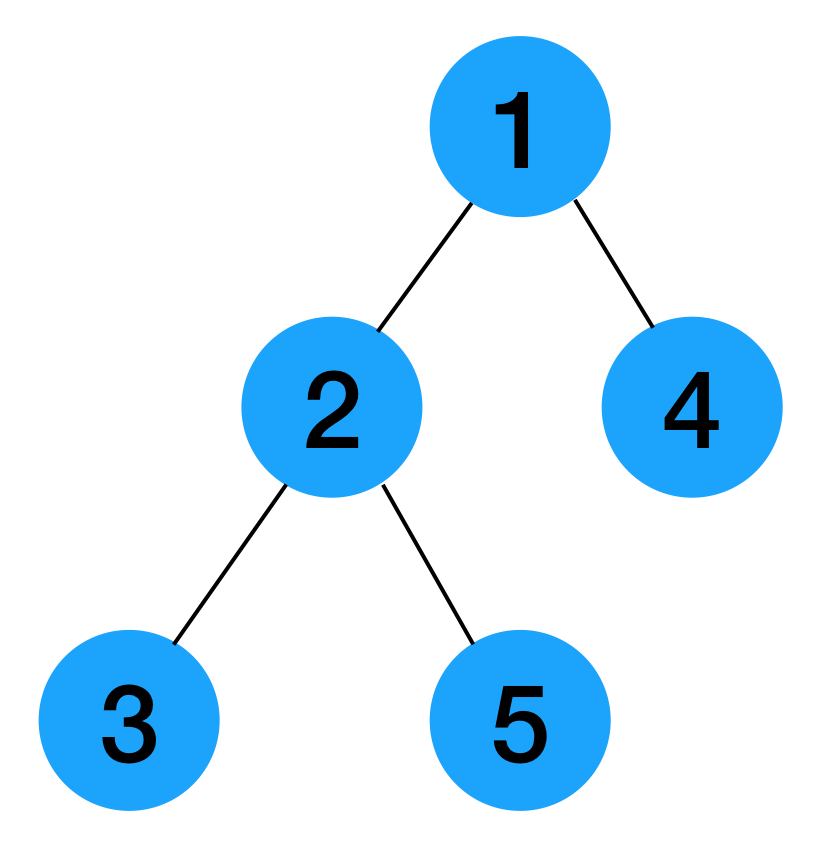
\includegraphics[scale=0.3,center]{pic1.png}

  File 5 is modified later than file 4 (since 5 is larger than 4, and thus file 5 has a later last modification timestamp, resulting in it being listed in a later position than file 4 in the command line arguments according to our assumption), but file 5 actually should not consider file 4 as one of its ancestor, because file 5 comes from modifications of file 2, and is on a editing path branch disjoint from that containing file 2. 

  But overall, our approach should work good enough. 
  \item The author of the files knows to separate each section, or paragraph of his files by an empty line. Like:
  \begin{lstlisting}
  <paragraph1>

  <paragraph2>

  <paragraph3>
  \end{lstlisting}
  This is not an unusual hypothesis and is actually how most English users format their documents as well as formatting languages such as LaTeX. 
\end{enumerate}
Now, when we open a certain file $i$, we want to be able to know:
\begin{enumerate}
  \item \textbf{Objective 1}: Amongst all the paragraphs of all files provided by our user, which paragraph is most likely to be the direct predecessor of this paragraph $j$? Or, which paragraph is most likely to be the direct source of modification for this paragraph?
  \item \textbf{Objective 2}: After finding the most likely predecessor of this paragraph, what are the minimum amount of edits required to change from the predecessor paragraph to the paragraph under inspection?
\end{enumerate}

Objective 2 as we described in the last subsection, is addressed by an optimized version of Edit Distance algorithm, which we call \texttt{BetterDiff}. Objective 1's on the other hand, is key to speeding up the application to a speed suitable for real-life usage. \\

We achieve Objective 1 by matching texts in the unit of paragraph first, which largely helps reduce the computational effort required. Yet this scheme does not violate any practical editing convention to render the application futile. Normally, when a user edits a file, the edits, however many at a time, can be each bucketed into its own paragraph. By matching paragraphs first, we limit the scope to apply \texttt{BetterDiff} on to only a paragraph a time.  This is analogous to an idea in 3D rendering that you don't have to calculate the effect of each object for the entire scene. You just have to render a small radius which affect viewpoint the most. This optimization can reduce the computational cost of the application by a factor as large as hundreds in practice. \\

The key idea behind implementing Objective 1, and the paragraph matching explained above, is to determine textual similarities. There is a well-established technique called MinHash which is used to calculate a string's signature, which can in turn be used to be compared with another string's signature to determine the similarity between the two documents. We used a third-party library \cite{minhash} which can return the similarity of two strings based on the MinHash algorithm. \\

There are more subtleties to be clarified in this scheme. But we shall leave further elaboration to later part of this document. 

\subsection{Running Instructions \& Presentation}
By this point, enough information is provided to understand what this project hopes to deliver. In this section, we provide step by step instructions so that you can run the application now and see the results before going further.\\

Our program \texttt{MDiff} takes a list of files as its input, the order of files within which as we mentioned before indicates the lastly-modified order from oldest to newest. It works in two mode, plain text patch file mode and HTML mode (enabled with \texttt{--html} flag). It generates a \texttt{.mpatch} or \texttt{.html} file for each file in the input. We process files by the their listed order, and each file are only compared with files before it, therefore no cycle is possible.\\

We have submitted packaged \texttt{jar} to be run directly. If you prefer to compile the source code yourself:
\begin{lstlisting}
$ mvn clean compile assembly:single
\end{lstlisting}

To use the program, suppose you have \texttt{1.txt, 2.txt, 3.txt} files in the folder, with filenames indicating order of their creation. Type in command line:
\begin{lstlisting}
$ java -jar MDiff.jar 1.txt 2.txt 3.txt
$ java -jar MDiff.jar --html 1.txt 2.txt 3.txt
\end{lstlisting}

\texttt{Mpatch} file is similar to \texttt{diff} result as we indent the file with two spaces and put block header around unoriginal content. If applicable, character changes are annotated below its line.
\begin{lstlisting}
= [filename]:[line number]
  Unchanged paragraph
---

< [filename]:[line number]
  Old content
  ---
> [current line number]
  New content
  +++
---
\end{lstlisting}
Recall the notion of editing chains mentioned before:\\
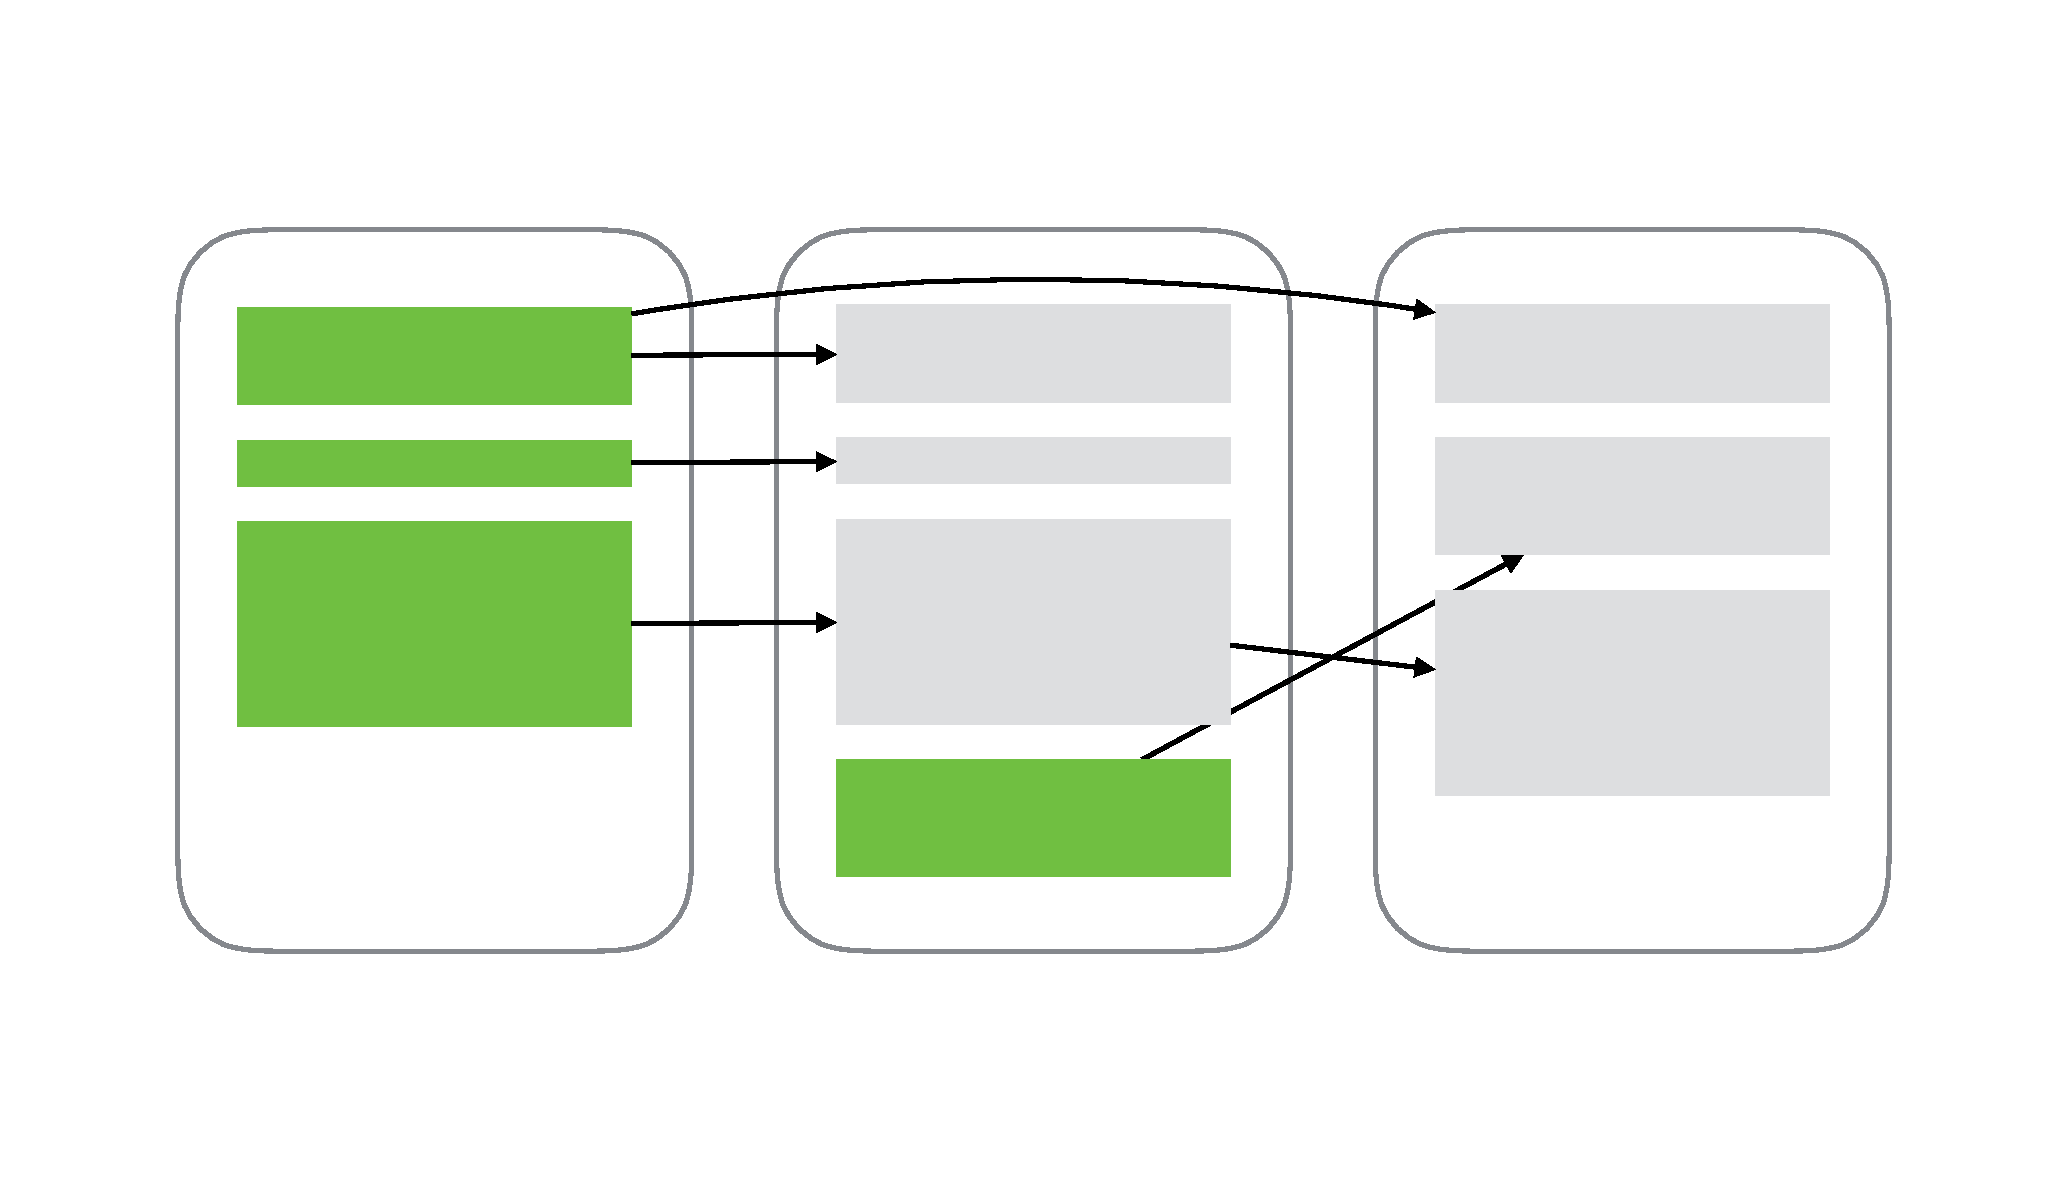
\includegraphics[scale=0.4,center]{1.pdf}\\

Here, each highlighted paragraph lies on the origin end of an arrow, which in itself marks a direct predecessor-successor relationship. That is, the paragraph at the end of the arrow comes directly from modifying the paragraph at the origin of the arrow.\\

To help illustrate \texttt{BetterDiff} at work, here is a picture displaying how the algorithm respects brackets pairing:\\
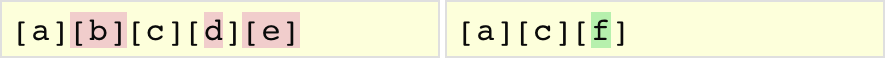
\includegraphics[center]{Screenshot1.png}\\

HTML version is a two column viewer where current file is displayed on the right. When you select a paragraph, its origin is displayed on the left, and changes from origin are annotated with color. The file that contains this clicked paragraph's predecessor shows up in the left column with the predecessor-successor paragraphs aligned as closely as possible. Matching paragraphs and \texttt{MDiff} edits are shown in corresponding colors. \\
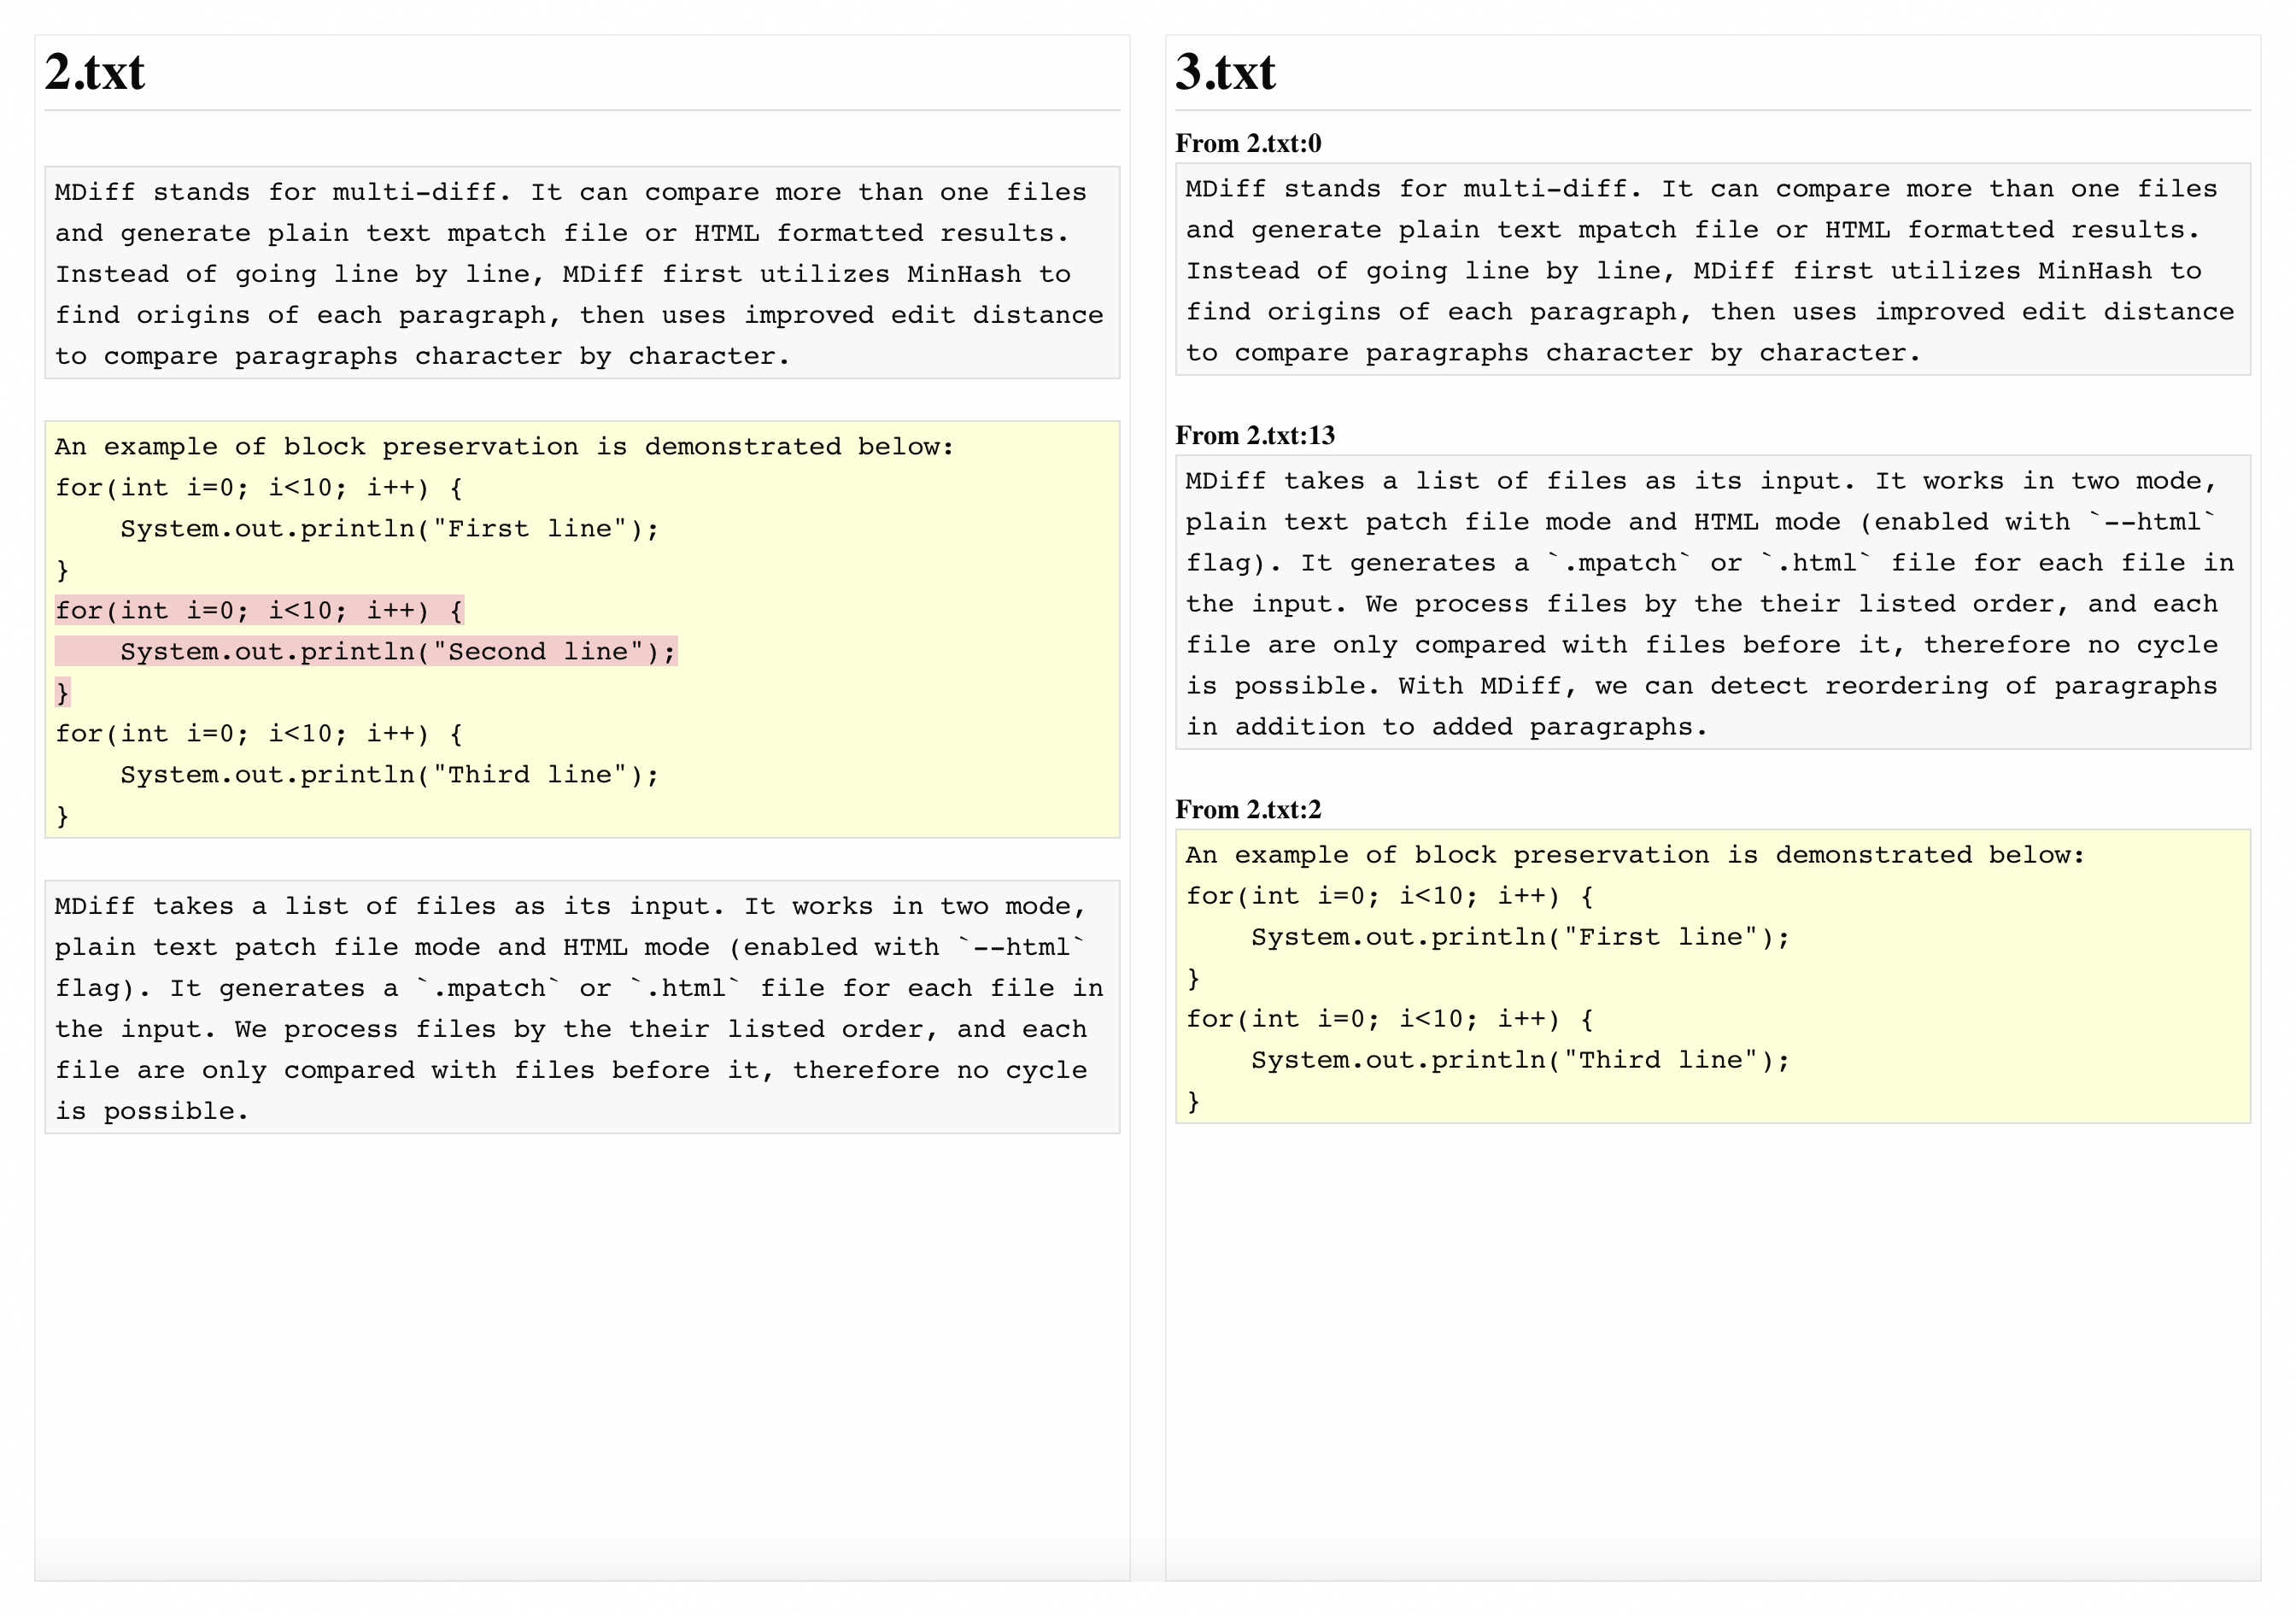
\includegraphics[scale=0.4,center]{Screenshot.png}\\

\pagebreak
\section{First Step: Predecessor Matching}
\textbf{Predecessor Matching} refers to the process of finding, for each paragraph $p$ in each file $file_p$, a paragraph that is most likely to be the origin of $p$ by virtue of having the largest pairwise similarity with $p$ amongst all the paragraphs that are contained in files coming before $file_p$. The concept of similarity is calculated by comparison of signature which is calculated by \textbf{MinHash}.
\subsection{Modelling}
As described in the previous section, our first goal is to be able to inspect a certain file $i$ in a sequence, and immediately locate the most similar paragraph amongst all files lastly-modified no later than this file, under assumptions:
\begin{enumerate}
  \item Files are given in time order from oldest to newest.
  \item The author of the files knows to separate each section, or paragraph of his files by an empty line. 
\end{enumerate}

The second assumption is established so that there is a valid way to define the notion of ancestry. If we treat an entire document as one single paragraph, then there is no point in saying \textit{finding the predecessor of this entire document}. Because in practice, most modifications between files are minor and of comparable degree, which means different successors of the same predecessor document may end up looking very much alike. Even if we devised an algorithm to locate such a predecessor document for the document being inspected, the output is most likely to be inaccurate and uninformative. \\

After dividing a document into paragraphs, the notion of ancestry and the concept of reusing now makes sense. Think it this way: when you write code, if you say \textit{reuse}, you usually refers to reusing a part of a code file, usually a function, or block. But in the case you want to reuse the code file in its entirety, you just \texttt{import} or \texttt{include} it. Such file-wise reusing operations would normally indicate the source of reusing directly and a dedicated algorithm to solve the ancestry relationship would be unnecessary. The same analysis applies to the case of general text files. We are only interested in finding the predecessor of a snippet of a text file, which is a reused part. There is no strict definition of delimitation of reused parts, obsession over which is moot per se. We conveniently pick up the convention of paragraph and delimit reusing in this sense. \\

Now, to find the most likely predecessor of a paragraph, is to find a paragraph that:
\begin{enumerate}
  \item is contained in a file earlier than the file that contains the paragraph under inspection.
  \item shares, amongst all paragraphs that satisfies the previous condition, a highest similarity with the paragraph under inspection.
  \item owns a similarity with the paragraph that satisfies the previous condition that is higher than a 80\% threshold.
\end{enumerate}
And to find such a paragraph that satisfies the above three conditions, we use the theory of textual similarity. \\

\subsection{Textual Similarity and Textual Signature}
Since this is only a subroutine we resort to in this project, rather than the project itself's primary focus, the introduction here is brief. MinHash is a hashing scheme that, instead of being as random as possible, provides locality sensitivity. Its hash result is called the \textit{signature} of this text. MinHash is designed to be able to hash similar texts to similar signatures. And by a corresponding comparison function of two texts' signatures, the two texts' similarity can be easily determined.

\subsection{Implementation}
Back to the implementation of the application. In particular, we implement the process as follows:
\begin{enumerate}
  \item Read in all files in the order provided by the user-specified command line argument list order. Create two string arrays, one to store the filenames of all the files in question and one to store each file's content of all files. 
  \item For each content string of the file content array, break up the content string into a string array to store this file's lines. By doing this, we have a 2-dimensional array of \texttt{filelines[m][n]} where \texttt{m} stands for the number of files involved, and \texttt{n} stands for each file's number of lines in its content. Then we trim out the tabs and whitespaces at the head and tail of each line. 
  \item Using this 2-dimensional array \texttt{filelines[m][n]}, we scan all the lines of all files, and break up all the lines into paragraphs by the delimiter of \textit{emptyline} as mentioned before. For each paragraph, we iterate through all paragraphs discovered before it, and find the one paragraph with the highest similarity to it, which has to be above 80\%. We determine this paragraph as the \textbf{predecessor} of current iteration's paragraph. Relevant information are all stored.
  \item Once we know the predecessor for each of all paragraphs of all files in the folder, we maintain the edit distance produced by the our \texttt{BetterDiff} algorithm with each paragraph. More specifically, this edit distance is calculated against each paragraph's predecessor with itself. By now, we have all the information we need to implement the application layer features in the future. For each paragraph, the information maintained, in summary, typically consists of:
  \begin{itemize}
    \item The file that contains this paragraph.
    \item The start and ending line numbers of this paragraph in the file that contains it. With these line numbers and the file number stored in the above entry, the paragraph itself can now be uniquely located.
    \item A reference to the paragraph's \textbf{predecessor}, which is determined by a concept of \textit{maximum similarity so far} as described above.
    \item Annotation to represent the result of running \texttt{BetterDiff} with this paragraph's predecessor as the first argument and this paragraph itself as the second argument. Note that although we are trying to accomplish something that looks like multi-file \texttt{diff}ing here, the \texttt{BetterDiff} algorithm itself only takes two strings at a time. 

    The annotation consists of three parts. We will illustrate each part's meaning with this example's help:
    \begin{lstlisting}
[a][b]
 -  -

[b][a]
 +  +
    \end{lstlisting}
    \begin{itemize}
      \item The \texttt{boolean same} value, which is \texttt{true} if the two string arguments are the same, which means the edit distance is 0. In the case of the example shown here, this flag should be \texttt{false}.
      \item The \texttt{boolean[] delete} flag array. The explanation is left below.
      \item The \texttt{boolean[] add} flag array. Remind yourself that although we are introducing the information maintained for each paragraph, the \texttt{delete} and \texttt{add} flag arrays actually apply to this paragraph's predecessor and this paragraph itself. This does not cause any confusion since for each paragraph, its predecessor can be uniquely identified.

      The \texttt{delete} boolean flag array corresponds to the predecessor string, which is \texttt{[a][b]} in this case. The flags in this array indicates whether each character in the string would be kept when the predecessor string is being edited into the target successor string with minimum editing distance. In particular, each flag is false if the corresponding character in this paragraph's predecessor paragraph should be deleted in min-distance editing. In this case, the \texttt{delete} array should be \texttt{\{true,false,true,true,false,true\}}. Note that this information is stored with the paragraph \texttt{[b][a]}, rather than the paragraph (string) \texttt{[a][b]}.

      Similarly, \texttt{add} boolean flag array corresponds to the new, or successor string/paragraph of the pair. If \texttt{add[i]} is true, then the character at 0-based position $i$ will be be seen as an \textit{unedited} character (\textit{unadded} in the particular case of the string being the successor) when trying to edit this paragraph's predecessor into this paragraph itself with minimum distance. If \texttt{add[i]} is false, then the character at position $i$ will be considered newly added during the min-distance editing. In this example, the \texttt{add} array, of a value \texttt{\{true,false,true,true,false,true\}}, should be maintained with the paragraph \texttt{[b][a]}. 

      Please pay attention to the similarity between \texttt{delete} and \texttt{add} in this example. Note that as long as the edits on each string occurs at the same location, the corresponding flag will be the same for either string, regardless the edit itself being \texttt{-} or \texttt{+}. That is, the flag value is determined only by the position of edits, not by the kind. This is a revelation peculiar to our implementation scheme, which will come handy later.
    \end{itemize}
  \end{itemize}
\end{enumerate}

This section is intended to focus on matching each paragraph with its predecessor, which is located by the \textit{most similar paragraph so far} scheme as decribed above. In the explanation, we assumed that we already have the utility of \texttt{BetterDiff} and includes its result for each paragraph together with the result of \textbf{Predecessor Matching}. Note that with these information stored, we can easily implement any visualization we want. We did implement a HTML-based visualization, but discussion shall be omitted. \\

Although this section is named the \textbf{First Step}, we essentially introduced the big picture architecture of the project. With the skeleton built out, all that left is to fill in the muscles, especially a powerful one. The \textbf{Predecessor Matching} scheme based on \textbf{MinHash} provides all the inter-paragraph information we need. To get the intra-paragraph information, we need an algorithm to compare a paragraph itself to its predecessor paragraph. And the introduction of this algorithm is developed next.

\pagebreak
\section{\texttt{BetterDiff}}
Our optimization of the original \texttt{diff}, or Edit Distance algorithm, focuses on fixing Edit Distance algorithm's ignorance of \textbf{brackets pairing}. Note that although we use the term \textit{brackets} here, we actually refer to parentheses, brackets, braces in general. This naming convention would apply for the rest of this document. \\

In section 1 of \textit{Introduction}, we gave an example where Edit Distance algorithm won't be able to find an optimal result. In our improved algorithm of \texttt{BetterDiff}, we are able to deal with not only ignorance of brackets pairing, which in practice usually comes in the form of an editing that deleted or added only part of a paring of brackets, but also the ignorance of quote pairing. Special scenarios like escaping character are also considered.

\subsection{Failed Attempt 1 with ZIMPL}
This problem appears to us in the beginning as difficult to solve with Dynamic Programming which is adopted by the original Edit Distance algorithm. We decided to put what we learned in this course in practice and give ZIMPL\footnote{\href{http://zimpl.zib.de}{\textcolor{blue}{ZIMPL} is a sophiscated mathematical programming language, a little language.}} a try. \\

The files associated with this attempt are all put in the folder \textit{Deprecated} which is located at the root level:
\begin{itemize}
  \item \texttt{Script.java} is a trivial Java file to write input \texttt{txt} files for the program. \texttt{out.txt} is the temporary file of the Java file's output.
  \item \texttt{old.txt} and \texttt{new.txt} are files to represent the old string and new string as the input of the program. Instead of expressing the inputs as a string, we expressed them as an array of integers. The encoding and decoding between should be straightforward.
  \item \texttt{zimpl\_attemp1.zpl} is the program file. I would not recommend running it since it unfinished and erroneous in nature. 
\end{itemize}

The approach we took in this attempt is to encode each input string's each character as an integer. Then we try to use ZIMPL to decide a binary variable for such a digit. This binary variable plays a role similar to each \texttt{delete} and \texttt{add} boolean flag we used in the java program. \\

The process should be easier to explain with an example. Note that in this attempt we have not come so far to addressing the ignorance of bracket pairing yet. Implementing Edit Distance alone seems difficult enough. With this simple example, we begin the discussion:
\begin{lstlisting}
Old String:
#index, number
1,1
2,2
3,3
4,4
5,5

New String:
#index, number
1,1
2,2
3,4
4,3
5,5
\end{lstlisting}
The input string is stored in variables \texttt{old[M]} and the output string is stored in variables \texttt{new[N]}. For \texttt{M}, we also have the binary annotation variable \texttt{delete[M]}, and similarly \texttt{add[N]} for \texttt{N}. Note that the value of the binary variables are the opposite of the \texttt{delete} and \texttt{add} Java boolean flags mentioned above. Here, \texttt{delete[m]} is 1 iff the digit $m$ of the input string (digit array) should be deleted in a min-distance editing. Similarly, \texttt{add[n]} should be 1 iff the digit $n$ should be seen as an added digit in a min-distance editing. \\

With such definition, we derive another two variable definitions: \texttt{after\_delete[M]} and \texttt{before\_add[N]}.  \texttt{after\_delete[M]} is essentially \texttt{old[M]} after a mapping function being applied, which sets \texttt{after\_delete[m]} to 0 if \texttt{delete[m]} is 1 and to \texttt{old[m]} otherwise. \texttt{before\_add[N]} is defined in a similar way. It is intuitive to add a minimizing objective function, where the coefficients of \texttt{delete[M]} and \texttt{add[N]} are all positive. All that's left to now is to set up constraints. \\

Note, to express that the editing determined by \texttt{delete[M]} and \texttt{add[N]} is a valid editing, we have to express applying the indicated editing would correctly transform \texttt{old[M]} to \texttt{new[N]}. Such a notion of valid editing shall be implemented with a constraint, which we might as well call \textbf{mapped equality} that could determine the following two strings equal (these two strings do conform to the example inputs listed above):
\begin{lstlisting}
after_delete[M]:
1,2,0,4,5

before_add[N]
1,2,4,0,5
\end{lstlisting}
This turned out to be hard. We first considered removing zeroes, which shortly turned out unpromising if we have a general case of \texttt{1,2,0,0,0,0,0,3,4} to process. We can't express the idea of a while-loop in ZIMPL, and it is infeasible to remove consecutive zeroes of arbitrary length. \\

Even more, at this point, we realized that trying to further transforming \texttt{after\_delete[M]} and \texttt{before\_add[N]} is very hard. We then turned our mind to tuning the objective function with some soft constraints to lure the solver to the correct solution. These attempts all failed with some input cases so I will just briefly summarize here:
\begin{itemize}
  \item Objective function: the terms
  \begin{lstlisting}
  sum <m> in M: delete[m] + sum <n> in N: add[n]
  \end{lstlisting}
   are fixed in all the approaches below. 
  \item Hard constraint: sum of \texttt{after\_delete[M]}  and \texttt{before\_add[N]} should be equal. This is only a necessary constraint to express the mapped equality, but not enough to be sufficient.
  \item Hard constraint: the number of zeroes in each of \texttt{after\_delete[M]} and \texttt{before\_add[N]} is the same. Again, this is also only a necessary constraint. \\

  And the below approaches are mostly inspired by analysis of concrete input cases:
  \begin{itemize}
    \item Approach 1: adding 
    \begin{lstlisting}
    - vabs(sum <m> in M: after_delete[m] * m - sum <n> in N: before_add[n] * n) / 2
    \end{lstlisting}
     to the objective function. However we tune the weight of this term, the solver would always be too eager to increase the number of deletions and additions to maximize its gain on this term.
    \item Approach 2: derive \texttt{difference1[M]} for \texttt{after\_delete[M]} with \texttt{difference1[m]} standing for \texttt{after\_delete[m-1]} minus \texttt{after\_delete[m]}. \texttt{difference2[N]} is defined similarly based on \texttt{before\_add[N]}. Then we require that:
    \begin{lstlisting}
sum <m> in M: vabs(difference1[m]) == sum <n> in N: vabs(difference2[n])
    \end{lstlisting}
    We did know this constraint can't be enough. Though seems tempting, the solver, for various input cases, ends up finding clever roundabouts satisfying this constraint. 
    \item Approach 3: \texttt{difference} variables defined as above. But now we add 
    \begin{lstlisting}
+ vabs(sum <m> in M: vabs(difference1[m])*m - sum <n> in N: vabs(difference2[n])*n)
    \end{lstlisting}
    To the objective function.
  \end{itemize}
  Other trivial approaches are tried out as well, and do not merit mentioning here. 
\end{itemize}


\subsection{Suboptimal Attempt 2 with ZIMPL}
Upon exploration, we realized that the difficulty of constraint expression mostly comes from the form of encoding we picked. Thus in this attempt, we changed to another approach of encoding the problem. The program associated with this attempt is stored in the \textit{Deprecated} subfolder as \texttt{zimpl\_attemp2.zpl}. \\

This attempt's code is better explained with an example (note that the explanations here are to be viewed together with the code. Some settings in the source code are not mentioned here for brevity of expression) :
\begin{lstlisting}
param s1[I2] := <1>10,<2>11,<3>12,<4>10,<5>13,<6>12 default 0;
param s2[I2] := <1>10,<2>11,<3>12,<4>10,<5>14,<6>12,<7>10,<8>13,<9>12 default 0;
\end{lstlisting}
These two sets of parameters refer to the input arrays. Thus, what we have as inputs here are:
\begin{lstlisting}
input1: 10, 11, 12, 10, 13, 12
input2: 10, 11, 12, 10, 14, 12, 10, 13, 12
\end{lstlisting}
The length parameter here is \texttt{l=max(6,9)=9}, and correspondingly:
\begin{lstlisting}
set I := {1..9}
set I2 := {1..18}
\end{lstlisting}
Why do we have \texttt{I2}? Because now instead of transforming each deleted or added digit to 0 explicitly, we implicitly express the edit as a digit not being chosen. Thus to express \texttt{1,2,3,4,5} with 3 deleted in the min-distance editing, we simply express \textit{we only choose digits at indices of \texttt{1,2,4,5,6}}. Note that the digit at index 6 here is out-of-bound, which is 0 by padding. And the existence of \texttt{I2} is exactly for this purpose. As long as we decides to delete some digit in the original legit index bound \texttt{I}, we express it as omitting the deleted digit's index, and adding alternatively another out-of-bound index in the padding region filled with 0s. Remind yourself that, adding in the second argument string can be viewed the same way as deleting a digit in the first argument string. This is illustrated before when we introduced the Java boolean flag arrays \texttt{delete} and \texttt{add}.\\

We first have variables \texttt{in1[I]} and \texttt{in2[I]}. Taking \texttt{in1[I]} as an example. \texttt{in1[1]} refers to the fact that the digit 1 is not affected (deleted) in the min-distance editing. All other \texttt{in1} and \texttt{in2} variables are defined similarly. Back to our example, we should have in an optimal solution:
\begin{lstlisting}
input1: 10, 11, 12, 10, 13, 12
in1:     1,  2,  3,  4,  5,  6
input2: 10, 11, 12, 10, 14, 12, 10, 13, 12
in2:     1,  2,  3,  7,  8,  9, 10, 11, 12 
\end{lstlisting}
The digits at indices 4, 5 and 6 of \texttt{input2} are deleted in the optimal solution, so \texttt{in2[4],in2[5],in2[6]} points to consecutive positions after the 3 deleted digits (technically they are ``added'' digits in the second argument string, but again, adding in the second argument can also be viewed the same way as deletion in the first argument string). \\

With this sorted out, other variables are either somewhat repetitive or self-explanatory. \texttt{c1[I]} and \texttt{c2[I]} refers to the picked digits as instructed by \texttt{in1} and \texttt{in2}:
\begin{lstlisting}
input1: 10, 11, 12, 10, 13, 12
in1:     1,  2,  3,  4,  5,  6
c1:     10, 11, 12, 10, 13, 12
input2: 10, 11, 12, 10, 14, 12, 10, 13, 12
in2:     1,  2,  3,  7,  8,  9, 10, 11, 12 
c2:     10, 11, 12, 10, 13, 12,  0,  0,  0
\end{lstlisting}
Note that the last three zeros of \texttt{c2} come from the out-of-bound padding area after \texttt{input2}. \\

The explanations for constraints and objective functions are thus omitted for brevity. Incidentally, we view 10 and 12 as a pair of brackets and the constraint to respect their pairing are expressed in the objective function. In essence, the trick this attempt adopts is using index to filter out digits that would otherwise be 0s after editing transformations. The zero digits in attempt 1 is hard to deal with because they can appear at arbitrary positions with arbitrary consecutive lengths. The trick here, using auxiliary index variables and padding, implicitly picked out all the digits, which would be non-zero in attempt 1, together in a consecutive manner. \\

Despite being educative in nature, this program does not perform good enough in practice. Two input strings of maximum length 9 resolved into 3332 variables and 4718 constraints and turns out to be requiring 3 seconds to solve already (with adequate hardware and latest version of solver). Imagine dealing with paragraphs across lines. \\

To this point, we are quite convinced of the unlikeliness of solving the problem with ZIMPL. Thus starting from next attempt, we went back to good o'l Dynamic Programming. The hope is to add modifications so that Dynamic Programming can address the pairing problem explicitly.

\subsection{Suboptimal Attempt 3 with Backward-Chaining Dynamic Programming}
We started by analyzing where the ordinary Edit Distance algorithm started to went astray. Consider this example:
\begin{lstlisting}
[a][b][c]
  ---
[a][c]
\end{lstlisting}
If running in a Backward-Chaining, or top-down manner, the Edit Distance algorithm will produce a result as shown above. The desired result instead is:
\begin{lstlisting}
[a][b][c]
   ---
[a][c]
\end{lstlisting}
The reason for the ED algorithm's malfunction is because the tail of \texttt{][c]} are identical in both strings, and thus the algorithm only starts considering editing when it comes from the tail of string 1 to the index 5 (0-based) of string 1.\\

A quick fix immediately comes to mind: we can force the algorithm to consider dropping \texttt{string1.charAt(6)}, which is a \texttt{]}. At this position, the solver faces a subproblem with both input strings' tail being \texttt{]}, which is a closing bracket. We add one case handling block to the algorithm so that when the algorithm sees two input strings with same ending, which is a closing bracket, the algorithm will try first dropping the two tails altogether at first, and then try dropping only the longest string's tail. And the algorithm compare the two probing's return values. If the latter probing's return value, which results from dropping only the tail of the longer input string, is smaller or equal(which is the case in this example shown above), we choose the latter probing's strategy instead of dropping both tails. \\

This is the major modification added to ED algorithm in this attempt, and the program does produce desirable results for quite a lot of test cases, include the original three-for-loop case mentioned in the Introduction section, which terminates in less than 1 second. Note that memoization is implemented in all discussions here and below. \\

But we eventually decided that this trick is too hacky to work generally. Plus, it is unlikely to be able to address the paring of quotes with this simple optimization.

\subsection{Final Attempt 4 with Forward-Chaining Dynamic Programming}
First, we do a 1-pass iteration of each input string. We store the position of each opening of closing brackets. More specifically, we store each pair of brackets in the form of \texttt{closingIndex -> openingIndex}. We consider the substring between \texttt{openingIndex} and \texttt{closingIndex} as a block enclosed by this pair. \\

Note that there is a subtlety. Consider this code snippet:
\begin{lstlisting}
// context1
for (header) {
    // body
}
// context2
\end{lstlisting}
In this situation, we have to move the \texttt{openingIndex} of the opening curly brace to the head of its line. This is because we have to always associate each for-loop's header with its body which is a block enclosed by a pair of curly braces. And our later algorithm depends on the ability to process each pair-enclosed block as a whole. By moving the opening curly brace's index ahead, we practically included the header inside the block. This prevents the algorithms from breaking the atomicity between the header and the block when processing.\\

Blocks enclosed by quotes are determined in a more subtle way, and the discussions are omitted here. \\

For the rest of discussion to make sense, consider this memoization table for the two input strings of \texttt{[a][c]} and \texttt{[a][b][c]}, respectively denoted as string 1 and string 2:\\
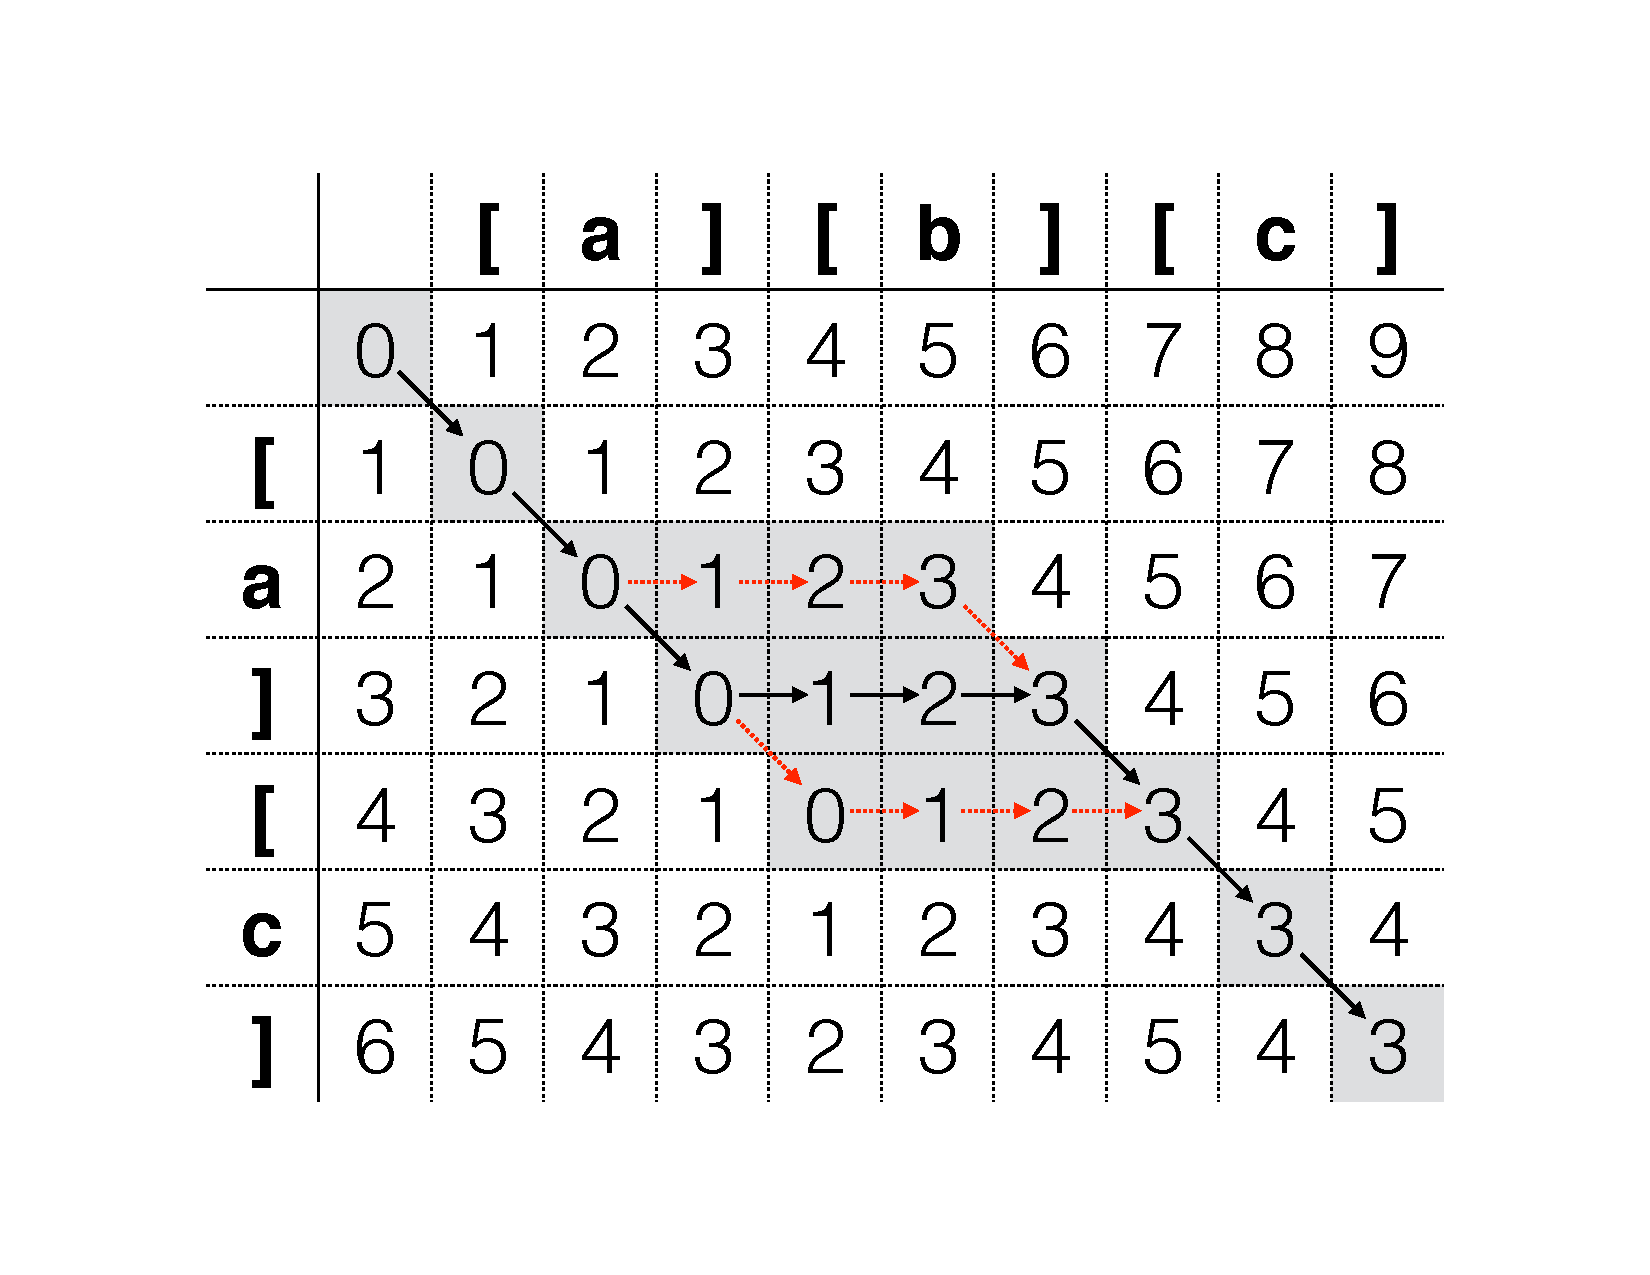
\includegraphics[scale=0.5,center]{2.pdf}\\

Note what we want to achieve here: in the middle region of this table, we have three paths. Using Forward-Chaining or Backward-Chaining, we would end up choosing either the path on the top or the path in the bottom. But what we really want here, is the path in the middle, which respects the pairing of the brackets. \\

Major modifications are in need to achieve this path control. We maintain, aside from a table \texttt{f[][]} as above, which shows the edit distance associated with each subproblem (indexed by the lengths of the two input argument strings), two other tables:
\begin{lstlisting}
private enum Direction { DIAGONAL, UP, LEFT }
...
Direction[][] prev = new Direction[s1.length + 1][s2.length + 1];
boolean[][] good = new boolean[s1.length + 1][s2.length + 1];
\end{lstlisting}
The first table \texttt{prev}, at each entry \texttt{prev[i][j]} stores how the \texttt{f[i][j]} edit distance is achieved. In particular, there are three ways of reaching \texttt{[i][j]}:
\begin{itemize}
  \item Moving down from its upstairs neighbor. In the table, if we choose to set \texttt{prev[4][5]} to \texttt{UP}, that would indicate that the algorithm should choose the result for the subproblem \texttt{\textbf{[a][} (compared with) \textbf{[a][b}} by deleting the character at index 4 of string 1. This is not possible in this case, but you should convince yourself about what each entry in \texttt{prev} means. In general, when an entry \texttt{prev[i][j]} is \texttt{DIAGONAL}, it means the tails of both input strings should be kept during editing. If it is either of the other two, which corresponds to horizontal or vertical moves, that means the algorithm has to delete (or add) one of the tails of the two strings.
  \item Moving right from its left neighbor. The analysis above applies similarly here. 
  \item Moving from the immediate top-left entry, which is \texttt{[i][j]}'s immediate previous diagonal neighbor. This means neither of the two strings' tails should be edited. 
\end{itemize}
The table \texttt{f[][]} and \texttt{prev[][]} all conform to decisions that a traditional Edit Distance algorithm would make. The third table \texttt{good[][]} on the other hand, means that it is possible to reach this entry without breaking any blocks as defined by enclosing pairings. Please refer to earlier parts of this section about how blocks are generated.\\

We won't bother you with a detailed step-by-step analysis of the algorithm, and will instead focus on being to the point here. The \textbf{loop invariant} here is:\\

At each entry \texttt{good[i][j]} is \texttt{true} iff on our way to reach this entry, we did so without breaking any pairs of brackets or quotes.\\

There are certain points that we should address here:
\begin{itemize}
  \item What does it mean to break a block? That means for the subproblem corresponding to \texttt{[i][j]}, this entry's solution's corresponding editing was not done without, for a certain pair of brackets, dropping one half in one input string's editing, while keeping both halves in another input string's output editing. That is to say, we require that for each pair of brackets, the two halves of the pair must either be both dropped in a sub-solution, or be both preserved in a sub-solution. Such an observation helps achieve what we set out to implement in the first place: fixing ignorance of brackets pairing.
  \item This invariant does not address the table \texttt{f[][]} and the table \texttt{prev[][]}. Again, these two tables store solutions that comes from dynamic decisions made in the same way as any bottom-up Dynamic Programming algorithm. 
\end{itemize}
With these revelations, it should be possible to relate to the code now. The major function is the \texttt{processCharacter} method in the \texttt{Distance.java} file. We provide a brief summary of how this function proceeds. Note that this function takes two strings and returns two \texttt{boolean[]} as annotation flag for each string. For each entry \texttt{[i][j]}, calculate the three estimates of edit distance from each of the \texttt{UP}, \texttt{DOWN} and \texttt{DIAGONAL} directions, and:
\begin{itemize}
  \item if any estimate is a strict minimum of the three, we determine this entry \texttt{[i][j]} comes from corresponding editing from that estimate's direction.
  \item If at least two of the three estimates are equal, that is no strict minimum exists, we pick amongst the three immediate neighbor of the three \texttt{UP}, \texttt{DOWN} and \texttt{DIAGONAL} directions one that provides an estimate no strictly larger than any other estimate and also is \texttt{good}. We set this entry \texttt{[i][j]}'s values for three tables according to editing from that neighbor. 
  \item If none of the three immediate neighbors is \texttt{good}, pick the \texttt{LEFT} one. 
\end{itemize}

In practice, the algorithm works well enough for the application to render the results we expected at inception of the project. 

\section{Conclusion}
Although we did not end up implementing the project using one of the declarative languages taught in the course, we did benefit enough from the algorithmic thinking cultured by courtesy of declarative reasoning. We also invented a little declarative language \texttt{mpatch} to describe file origin. This project so far is not perfect, and we unequivocally believe that there are input cases that could break our application and algorithm. But for this moment, we think we have made solid progress on improving a legacy algorithm. 






\begin{thebibliography}{9}
%The \bibitem is to start a new reference.  Ensure that the cite_key is
%unique.  You don't need to put each element on a new line, but I did
%simply for readability.
    \bibitem{minhash}
      \href{https://github.com/codelibs/minhash}{codelibs/minhash: A third-party Java-based library  for b-bit MinHash algorithm}


\end{thebibliography} %Must end the environment


\end{document}  %End of document.